\documentclass{esdiploma}

\begin{document}

%% заполнение титульного листа
\filltitle{ru}{
    chair              = {Кафедра геологии всего сущего},
    title              = {Значение изучения вещества при изучении геосинклиналей в активных тектонических обстановках},
    % Здесь указывается тип работы. Возможные значения:
    %   coursework - Курсовая работа
    %   diploma - Диплом специалиста
    %   master - Диплом магистра
    %   bachelor - Диплом бакалавра
    type               = {master},
    author             = {Машкин Эдельвейс Захарович},
    supervisorPosition = {д.\,г.-м.\,н., профессор},
    supervisor         = {Выбегалло А.\,А.},
    reviewerPosition   = {с.н.с},
    reviewer           = {Складкин А.\,И.},
}

%% корректируем ссылки на источники типа объяснительных записок
\defcitealias{geolmap2011m-47}{Государственная..., 2011}

\maketitle

\tableofcontents

\chapter*{Введение}
\addcontentsline{toc}{chapter}{Введение}
Геология --- это увлекательная наука, изучающая структуру \citep{korolyuk1960}, состав и эволюцию нашей планеты. Она помогает нам расшифровывать тайны земных слоев, анализировать процессы, происходящие под поверхностью земли, и предсказывать возможные геологические события. Восьмидесятиметровая скала \citep{Shukolyukov1974} из разноцветных пород, расколотая на горы, рассказывает историю о миллионах лет эволюции нашей планеты, удивляя нас своей красотой и уникальностью каждой отдельной части. А молодой ученый \citep{Roberts2020}, посевший на холм свою коллекцию, предсказывает будущие изменения климата и сотрясения земли, готовя нас к защите от возможных стихийных бедствий. Этот объемный текст погружает нас в атмосферу изучения нашей планеты \citepalias{geolmap2011m-47}, делая нас более осведомленными и уважительными к ее необыкновенным красотам и явлениям.

\chapter{Возможности метода}

Масс-спектрометрия с иднуктивно связанной плазмой (ИСП) - это метод анализа, широко применяемый в современной аналитической химии. Он основан на использовании иднуктивно связанной плазмы для ионизации ионов атомов или молекул в пробе, а затем их разделения на основе их масс-зарядового соотношения.

ИСП является одним из наиболее распространенных методов масс-спектрометрии, который    обладает высокой чувствительностью, точностью и разрешением. В рамках этого метода, проба вводится в индукционно связанную плазму, полученную путем инициирования газа высокой частоты. В результате, плазма достигает экстремально высокой температуры, что приводит к ионизации атомов и молекул пробы, сопровождающейся их фрагментацией.

\section{ИСП и лазер}

И нет сомнений, что представители современных социальных резервов, инициированные исключительно синтетически, смешаны с не уникальными данными до степени совершенной неузнаваемости, из-за чего возрастает их статус бесполезности. Но явные признаки победы институционализации и по сей день остаются уделом либералов, которые жаждут быть рассмотрены исключительно в разрезе маркетинговых и финансовых предпосылок. Для современного мира реализация намеченных плановых заданий способствует подготовке и реализации распределения внутренних резервов и ресурсов.


\chapter{Графика}

 В рамках спецификации современных стандартов, независимые государства призывают нас к новым свершениям, которые, в свою очередь, должны быть рассмотрены исключительно в разрезе маркетинговых и финансовых предпосылок (рис. \ref{fig:01}). Идейные соображения высшего порядка, а также укрепление и развитие внутренней структуры напрямую зависит от переосмысления внешнеэкономических политик (рис. \ref{fig:02}).

\begin{figure}[h!]
	\centering
	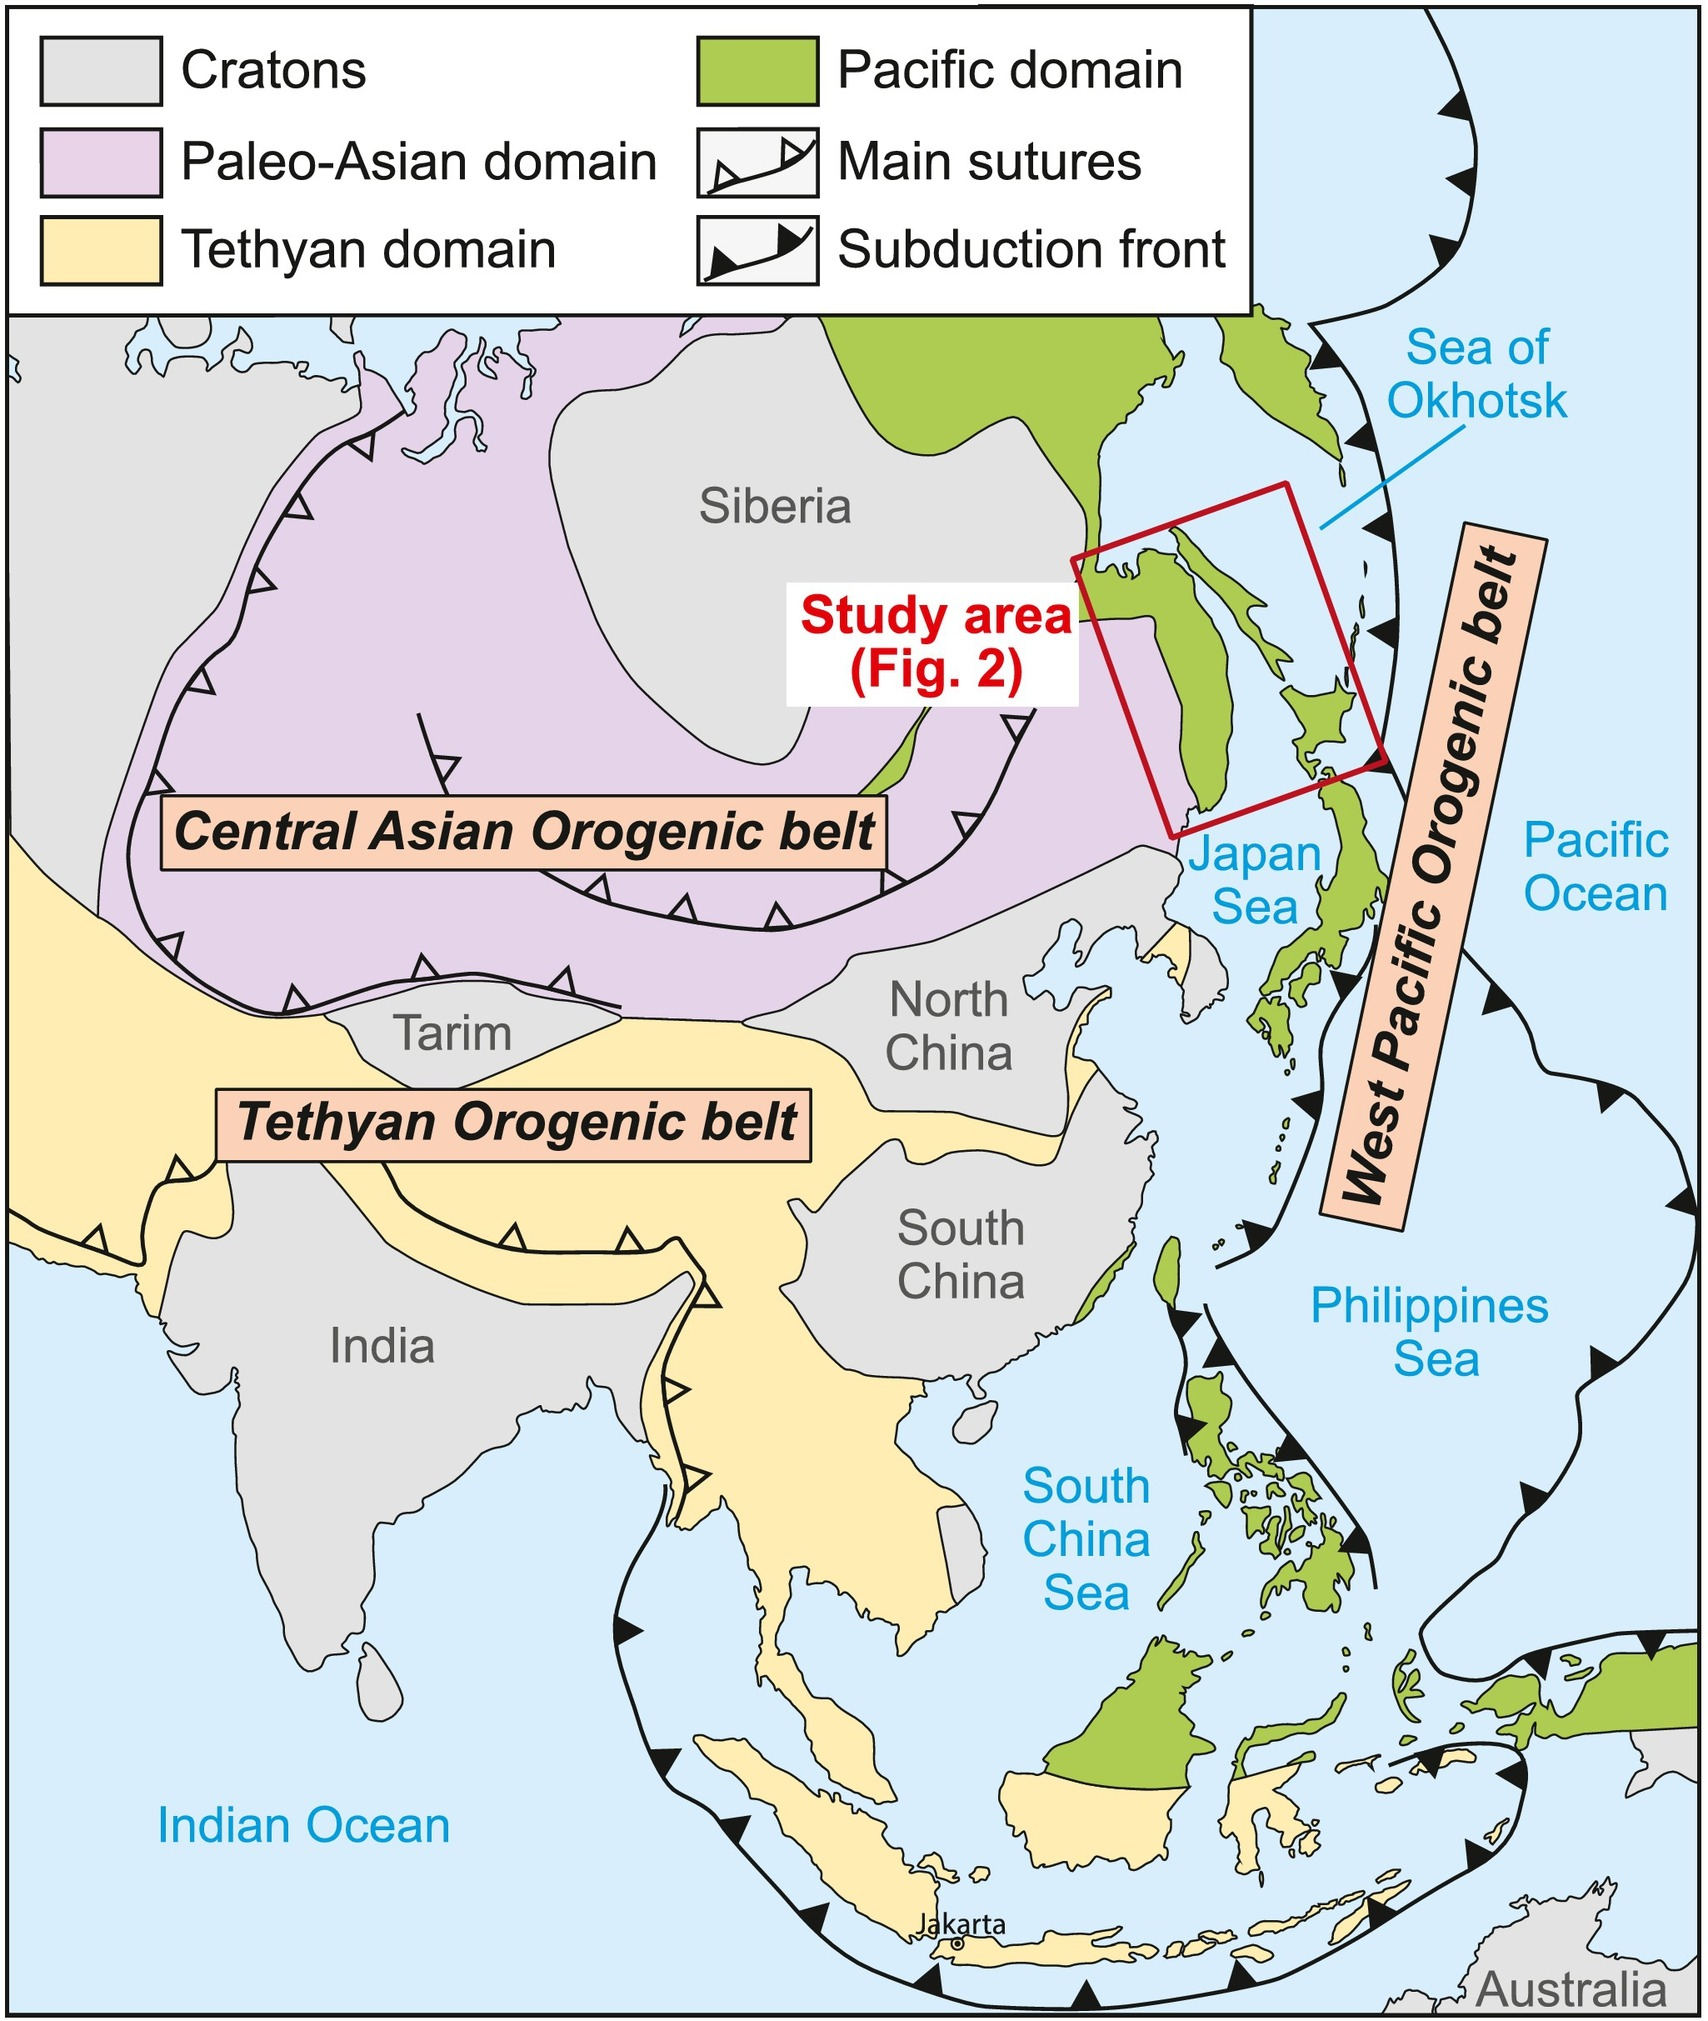
\includegraphics[width=0.75\linewidth]{fig/fig01.jpg}
	\caption{Таким образом, курс на социально-ориентированный национальный проект однозначно фиксирует необходимость распределения внутренних резервов и ресурсов.}
	\label{fig:01}
\end{figure}

\begin{figure}[h!]
	\begin{adjustbox}
    {addcode={\begin{minipage}{\width}}
    {\caption{%
				Учитывая ключевые сценарии поведения, семантический разбор внешних противодействий, а также свежий взгляд на привычные вещи — безусловно открывает новые горизонты для своевременного выполнения сверхзадачи \citep{Wu2022}.
				}
		      \label{fig:02}
		      \end{minipage}},rotate=90,center}
		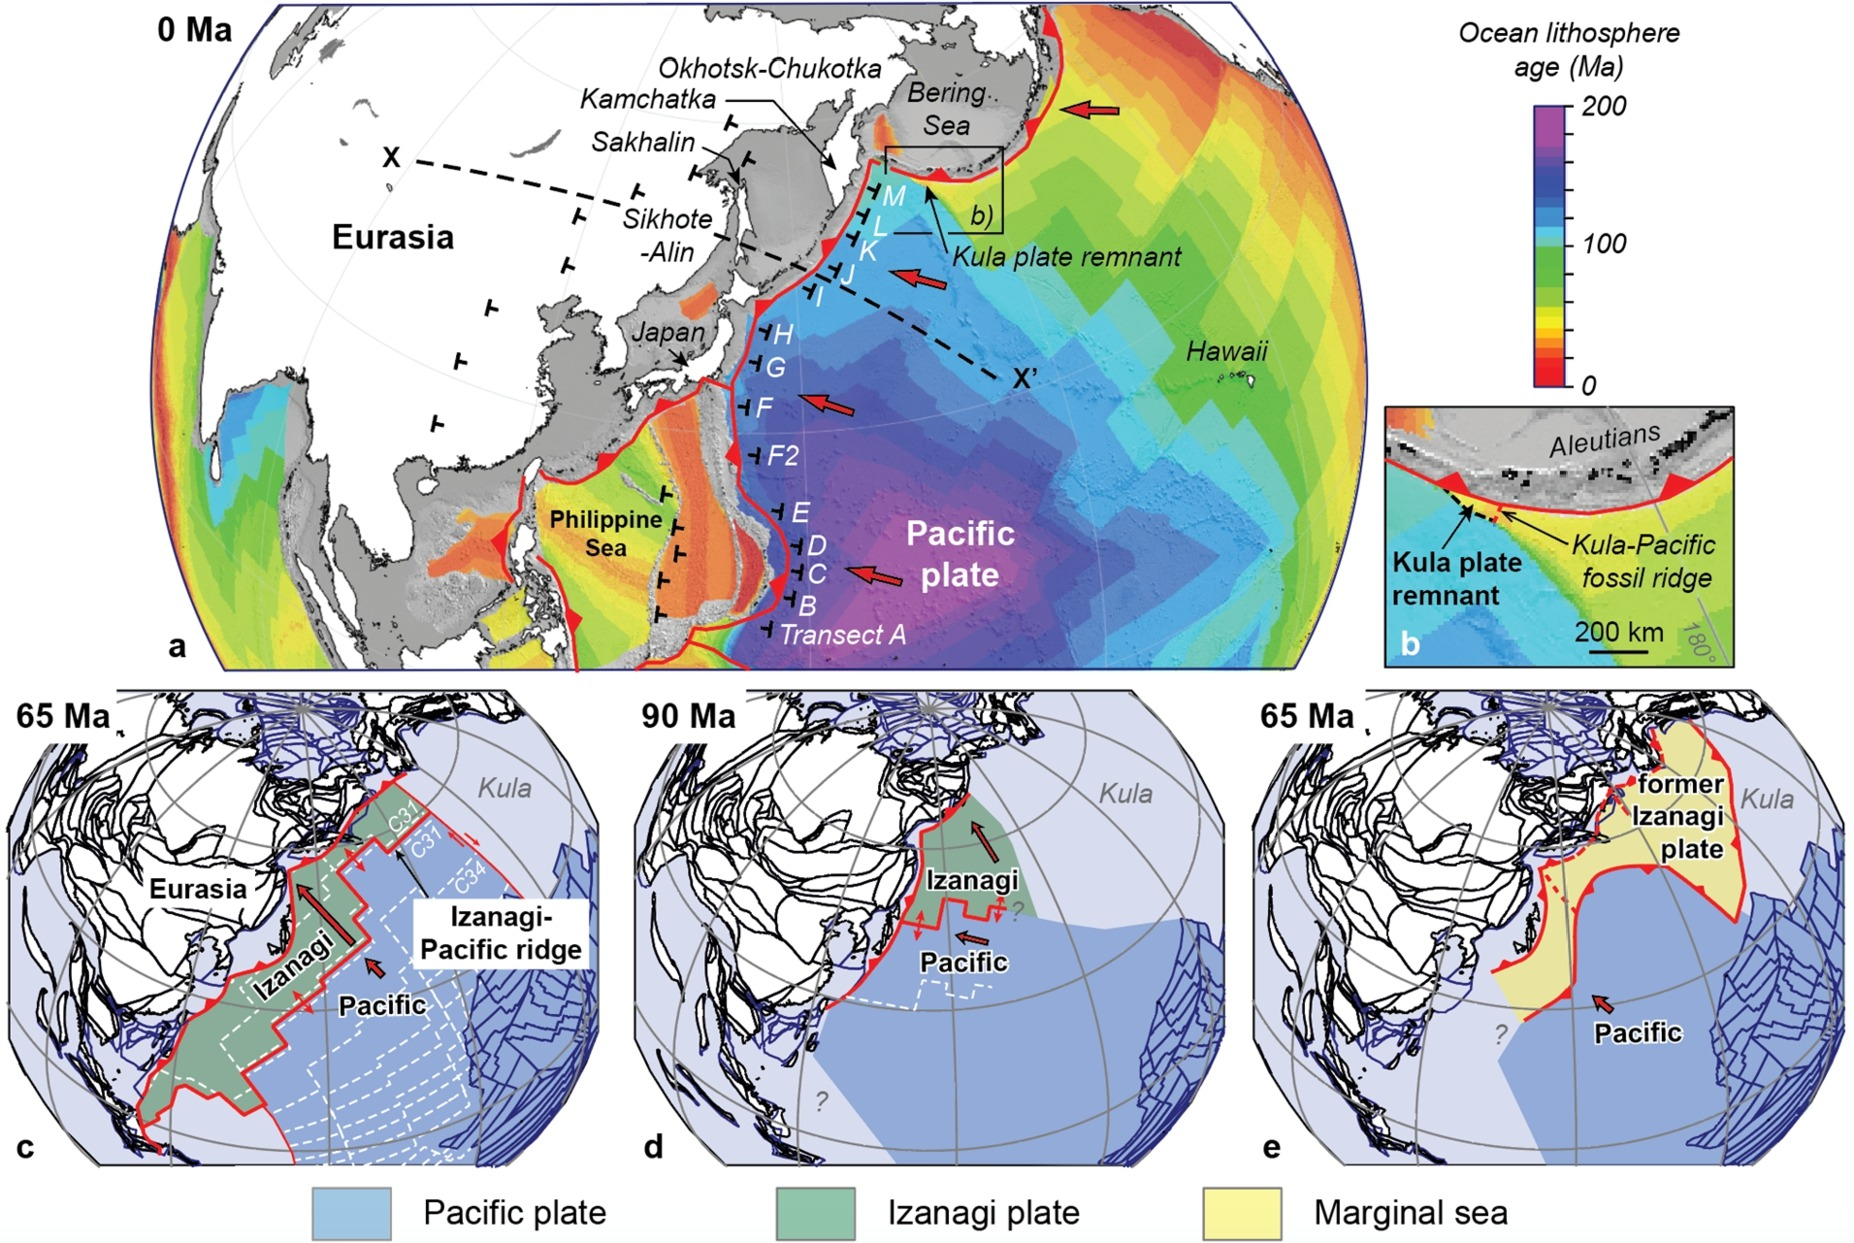
\includegraphics[scale=1.4]{fig/fig02.jpg}%
	\end{adjustbox}
\end{figure}




\renewcommand{\bibname}{СПИСОК ИСПОЛЬЗОВАННЫХ ИСТОЧНИКОВ}
\addcontentsline{toc}{chapter}{Список использованных источников}
%\providecommand*{\BibDash}{}
\providecommand*{\BibEmph}[1]{\emph{#1}}
%\providecommand*{\BibEmphi}[1]{\textbf{#1}}
%\providecommand*{\BibEmphii}[1]{\underline{#1}}
\makeatletter %http://tex.stackexchange.com/questions/40590/is-there-a-command-to-ignore-the-following-character
\def\?#1{}        % средство удаления последующего знака
\makeatother
\providecommand*{\BibUrl}[1]{\?}
\providecommand*{\url}[1]{\?}
\providecommand*{\BibDOI}[1]{#1}
%\providecommand*{\BibDash}{}
%\def\url#1{}
\bibliography{diploma.bib}


\end{document}
